

\documentclass[a4paper]{scrartcl}

% Mathematik-Pakete
\usepackage{amsmath}
\usepackage{amssymb}
\usepackage{amstext}
\usepackage{amsfonts}
\usepackage{mathrsfs}
\usepackage{paralist}
\usepackage[pdftex]{graphicx}
\usepackage{fancyhdr}
\usepackage{color}
\newcommand{\qed}{\begin{flushright}
$\blacksquare \dagger$ \end{flushright}}


%\usepackage[ansinew]{inputenc}
%\usepackage[T1]{fontenc}

\usepackage[utf8]{inputenc}
%\usepackage[latin1]{inputenc}  
\usepackage[T1]{fontenc}
%\usepackage{lmodern}          
\usepackage[a4paper]{geometry}
\geometry{verbose,tmargin=1.5cm,lmargin=2cm,rmargin=2cm,bmargin=2cm,nohead}
\usepackage[ngerman]{babel}
\setlength{\parindent}{0cm}


\begin{document}
\pagestyle{fancy}
\setlength{\footskip}{10mm}
\fancyhf{}
\renewcommand{\headrulewidth}{0pt}
\renewcommand{\footrulewidth}{0.5pt}

%\twocolumn[
 \centerline{\LARGE \bf \textsf{MSE CFD}} 
 \smallskip
\centerline{\Large \bf \textsf {Zusammenfassung}}
\medskip
  \centerline{\bf \textsf{dstrebel, s1bischo, sboller }}

 \smallskip \noindent\rule{\textwidth}{0.5pt}
\smallskip%]

\section{Introduction}
In dieser Zusammenfassung werden die Fragen vom Fragekatalog beantwortet.


\section{Conservation laws of fluid motion and boundary conditions}
\subsection{Conservation Euqations}
Explain the physical meaning of the different terms in the conservation
equations (link between mathematical “operations” and physical behaviour)

Präsentation Folie 7

Impulsgleichung


Energiebilanz

\begin{table}[h]
\begin{center}
\begin{tabular}{|l|l|}
\hline Continuity & $\frac{\partial(\rho)}{\partial t}+\operatorname{div}(\rho
\vec u)=0$
\\
\hline x-Momentum & $\frac{\partial(\rho u)}{\partial
t}+\operatorname{div}(\rho u \vec u) = - \frac{\partial p}{\partial
x}+\operatorname{div}(\mu \operatorname{grad} u)+S_{Mx}$ \\
\hline y-Momentum & $\frac{\partial(\rho v)}{\partial
t}+\operatorname{div}(\rho v \vec u) = - \frac{\partial p}{\partial
y}+\operatorname{div}(\mu \operatorname{grad} v)+S_{My}$ \\
\hline z-Momentum & $\frac{\partial(\rho w)}{\partial
t}+\operatorname{div}(\rho w \vec u) = - \frac{\partial p}{\partial
z}+\operatorname{div}(\mu \operatorname{grad} w)+S_{Mz}$ \\
\hline Energy & $\frac{\partial(\rho i)}{\partial
t}+\operatorname{div}(\rho i \vec u) = -p \operatorname{div} \vec u +
\operatorname{div}(k \operatorname{grad} T) + \Phi + S_i$ \\
\hline Equations of State & $p=p(\rho, T)$ und $i=i(\rho, T)$ \\
\hline
\end{tabular}
\caption{Governing Equation of the flow of a compressible Newtonian fluid}
\end{center}
\end{table}


\subsection{Explain the physical meaning of the different terms in a general
transport equation}

\begin{align}
\frac{\partial(\rho \phi)}{\partial t} + \operatorname{div}(\rho\phi\vec
u)=\operatorname{div}(\Gamma \operatorname{grad} \phi) + S_\phi
\end{align}

\begin{table}[h]
\begin{center}
\begin{tabular}{|p{3cm}|p{3cm}|p{3cm}|p{3cm}|}
\hline Rate of increase of $\phi$ of fluid element +& Net rate of flow of $\phi$
out of fluid element =& Rate of increase of $\phi$ due to diffusion +& Rate of
increase of $\phi$ due to sources \\
\hline Zeitliche Änderung von $\phi$  +& Konvektiver Transport: Fluss von $\phi$
mit der Strömung =& Diffusiver Transport: Transport von $\phi$ aufgrund von
Konzentrationsunterschieden (grad). Diffusionskonstante $\Gamma$ bestimmt Menge
+& Quellterm innerhalb des Fluidelements \\
\hline
\end{tabular}
\caption{Meaning of general transport equation}
\end{center}
\end{table}





\section{Turbulence and its modelling}

\subsection{Properties of turbulence}
Explain the properties of turbulence and their influence on the flow
field. Which changes can be observed compared to laminar flow?

\textbf{Turbulence is irregular, disorderly, non-stationary, three-dimensional,
highly non-linear, irreversible phenomenon}

\begin{itemize} 
\item Nichtlinear
\item Zufälligkeit (nicht Reproduzierbar)
\item 3D, auch wenn Mittelwert in 1D und 2D variert
\item hohe Wirbelstärke $\Rightarrow$ Energie wird transportiert.
\item Energie wird dissipiert (wird immer kleiner)
\item Intermittency: Turbulenz kann nur in Teilen der Strömung vorhanden sein.
$\Rightarrow$ Eine Strömung kann nicht nur aus turbulenten Anteilen bestehen.
\item Hohe Diffusivität von Impuls und Energie (Gute Verteilung)
\item Turbulenz ist lokaler Umgebung abhängig (z.B. Absatz)
\end{itemize}
\subsection{RANS and LES Modelling}
Explain the main approximations using RANS
and LES modelling, including assumptions (what is computed and how, what is modelled and how)
\subsubsection{RANS}
\textbf{Reynolds-averaged Navier–Stokes (RANS)}

\begin{figure}[h]
\begin{center}
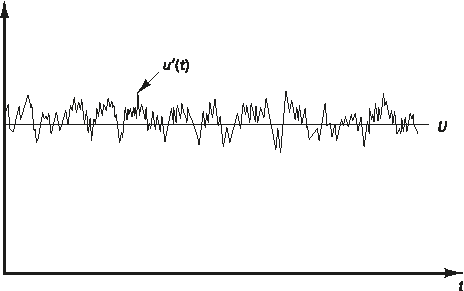
\includegraphics[scale=1]{images/51.pdf}
\caption{RANS Strömung}
\label{fig:41}
\end{center}
\end{figure}

RANS besteht aus einem Mittelwert der Strömungskennwerte und einem stochastisch
fluktuierenden Anteil. Vor der numerischen Berechnung der Lösung liegen die
Navier-Stokes Gleichungen als zeitgemittelt vor. Nichtlineare Extraterme liegen
in den RANS aufgrund der Interaktionen der verschiedenen turbulenten Fluktuationen vor.
Diese werden normalerweise mit klassischen Turbulenzmodellen wie dem
$k-\epsilon$- oder dem Reynoldsstress-Modell modelliert.
\\
\textit{Vorteile:} erträgliche Rechenleistung bei brauchbaren Resultaten,
deshalb die meistverwendete Methode. \\
\vspace{0.5cm}
\textbf{Large Eddy Simulation}
Nur grosse Turbulenzelemente werden exakt aufgelöst. Kleinere Turbulenzelemente
werden über Filterfunktionen herausgefiltert. Diese nicht direkt berechneten
Elemente werden über sogenannte Subgrid-Scale Models approximiert. \\
\vspace{0.5cm}
\textit{Vorteile:} Bessere Resultate insbesondere bei komplexen Geometrien. \\
\textit{Nachteile:} Grösserer Speicher- und Rechenzeitbedarf

\colorbox{red}{k-$\epsilon Modell$ und Bischi LES Bild, Lektion 12 Blatt}


\subsection{Wallfunctions} 
What are wall functions, idea behind them, advantages
and disadvantages.

Im Engineeringbereich interessieren die Details der Near-Wall Region im
Normalfall nicht. Von Interesse ist hingegen der Strömungswiderstand in der Nähe
der Wände. Wallfunktionen korrigieren die

Gleiche Anzahl Knoten, Strömung muss nicht über allzu feines Netz approximiert
werden. $\Rightarrow$ Spart Rechenleistung bei akkuraten Resultaten.\\

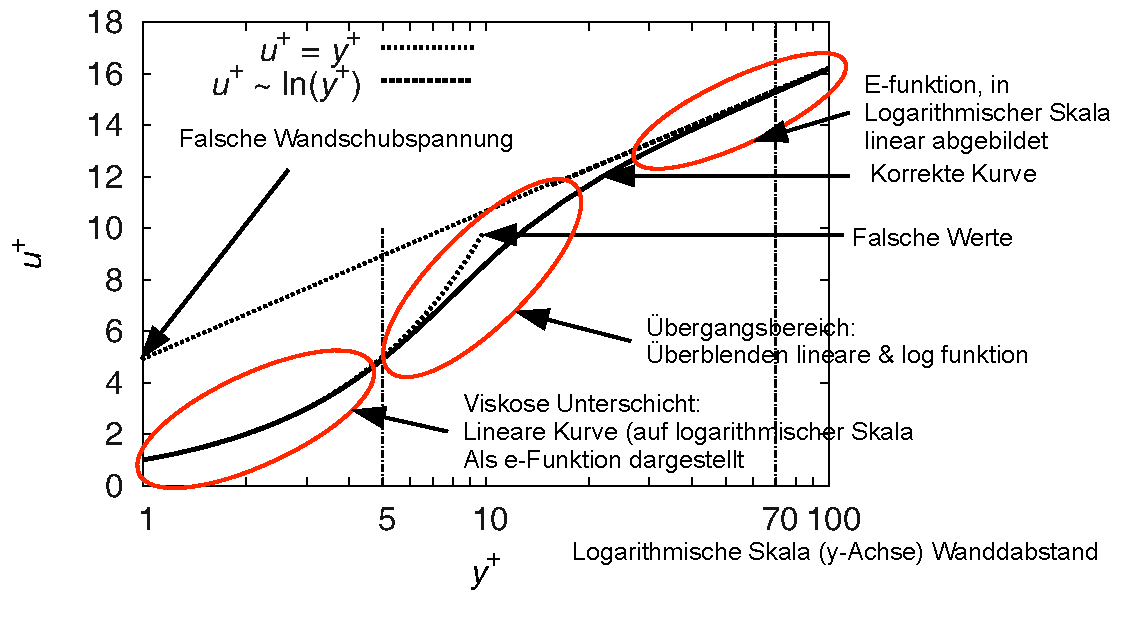
\includegraphics[scale=0.8]{images/wall_function.pdf}
% cut with: pdfcrop --margins '5 5 5 20' in.pdf out.pdf

\colorbox{red}{isch das klar?, bischsil}

\section{The finite volume method for the diffusion problem}


\subsection{FV Discretisation for a one-dimensional heat conduction Problem}
\subsubsection{Problemstellung}
Derive a finite-volume discretization for a one-dimensional heat conduction
problem. 

\begin{figure}[h]
\begin{center}
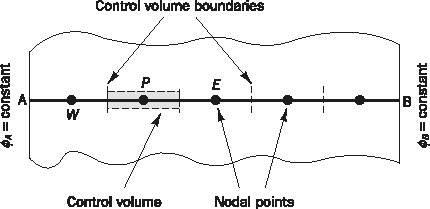
\includegraphics[scale=1]{images/41.pdf}
\caption{One-Dimensional Heat Conduction Problem}
\label{fig:41}
\end{center}
\end{figure}
Zur Diskretisierung wird das Gebiet in Kontrollvolumen geteilt. Bei diesem
Problem werden die Kontrollpunkte gleich zwischen den Randpunkten A und B
verteilt.

 Dieses Problem ist Steady-State und besteht nur aus dem Diffusionsterm der
 generellen Transportgleichung:
 
 \begin{align}
 \frac{d}{dx} \left( \Gamma \frac{d\phi}{dx}\right) + S = 0
 \end{align}
 \qed

\subsubsection{Diskretisierung}


\begin{figure}[h]
\begin{center}
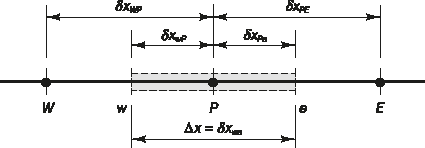
\includegraphics[scale=1.2]{images/42.pdf}
\caption{One-Dimensional Heat Conduction Diskretisierung}
\label{fig:42}
\end{center}
\end{figure}

Generell wird jeweils ein Punkt P wie in Abbildung \ref{fig:42} gezeigt
betrachtet. Rechts davon befindet sich ein weitere Kontrollpunkt genannt E für
East. Analog dazu befindet sich links der Punkt W. Klein e und klein w sind die
Kopfflächen des Kontrollvolumen dar. Die verschiedenen Abstände sind jeweils mit
einen $\delta$ bezeichnet.

Der wichtigste Schritt der FVM ist die Integration der das Problem
beschreibenden Formel. Dies geschieht für den Punkt P folgendermassen:

\begin{align}
\int_{\Delta V} \frac{d}{dx} \left( \Gamma \frac{d\phi}{dx}\right)dV +
\int_{\Delta V}SdV = \left(\Gamma A
\frac{d\phi}{dx}\right)_{e}-\left(\Gamma A \frac{d\phi}{dx}\right)_w +
\bar{S}\Delta V = 0
\end{align}
A ist in dieser Formel die Querschnittsfläche des Kontrollvolumens und $\bar{S}$
der Quellenwert des betrachteten Kontrollvolumen. Ein Vorteil dieser Methode ist
die klare physikalische Bedeutung: Der diffusive Fluss von $\phi$ der das
Kontrollvolumen auf der Ostseite verlässt minus der diffusive Fluss von $\phi$
der in das Kontrollvolumen auf der Westseite gelangt ist gleich der Quelle von
$\phi$ im Kontrollvolumen.

Die Werte von $\Gamma$ an den Stirnflächen e und w werden linear zwischen den
beiden Punkten E und W approximiert:

\begin{align}
\Gamma_w=\frac{\Gamma_W+\Gamma_P}{2} \\
\Gamma_e=\frac{\Gamma_P+\Gamma_E}{2}
\end{align}

Die Ableitungen $\phi$ werden ebenfalls linear über die Distanz $\delta x_{PE}$
und $\delta x_{WP}$ zwischen P und e bzw. w interpoliert.

\begin{align}
\left(\Gamma A \frac{d\phi}{dx}\right)_e = \Gamma_e A_e
\left(\frac{\phi_E - \phi_P}{\delta x_{PE}}\right)
\end{align}
\begin{align}
\left(\Gamma A \frac{d\phi}{dx}\right)_w = \Gamma_w A_w
\left(\frac{\phi_P - \phi_W}{\delta x_{WP}}\right)
\end{align}

Der Quellterm wird meistens als Funktion der abhängigen Variable dargestellt:

\begin{align}
\bar{S}\Delta V = S_u+S_p\phi_P
\end{align}


Gesamthaft ergibt sich folgende Formel für das betrachtete Kontrollvolumen:

\begin{align}
\Gamma_e A_e \left(\frac{\phi_E-\phi_P}{\delta x_{PE}}\right)-\Gamma_w A_w
\left(\frac{\phi_P-\phi_W}{\delta x_{WP}}\right)+(S_u+S_p\phi_P)=0
\end{align}

oder nach Umstellung:
\begin{align}
\boxed{\left(\frac{\Gamma_e}{\delta x_{PE}}A_e + \frac{\Gamma_e}{\delta
x_{WP}} A_w -S_p\right)\phi_P=\left(\frac{\Gamma_w}{\delta x_{WP}}A_w\right)
\phi_W + \left(\frac{\Gamma_e}{\delta x_{PE}}A_e\right)\phi_E+S_u}
\end{align}

In Koeffizientenschreibweise:

\begin{align}
\boxed{a_P\phi_P=a_W\phi_W+a_E\phi_E+S_u}
\end{align}

\qed
\subsection{Taylor CDS Second Order}
Demonstrate, using Taylor series expansion, that the central differencing scheme
has second order accuracy.\\
\textbf{Taylorentwicklung von $\mathbf{\phi}$} \\

\begin{align}
\boxed{\phi_E=\phi_P+\phi'\delta x_{PE} + \frac{1}{2}\phi''\left(\delta
x_{PE}\right)^2+\frac{1}{6}\phi'''\left(\delta x_{PE}\right)^3\ldots}
\end{align}

\begin{align}
\boxed{\phi_W=\phi_P-\phi'\delta x_{WP} + \frac{1}{2}\phi''\left(\delta
x_{WP}\right)^2-\frac{1}{6}\phi'''\left(\delta x_{WP}\right)^3\ldots}
\end{align}

\begin{align}
\Gamma_e A_e \left(\frac{\phi_E-\phi_P}{\delta x_{PE}}\right)-\Gamma_w A_w
\left(\frac{\phi_P-\phi_E}{\delta x_{WP}}\right)
\end{align}

\begin{align}
\Gamma A \left(\phi' + \frac{1}{2} \phi''\delta
x_{PE}+\frac{1}{6}\phi'''\left(\delta x_{PE}\right)^2\right) + \Gamma A
\left(-\phi'+\frac{1}{2}\phi''\delta x_{WP} - \frac{1}{6} \phi'''
\left(\delta x_{WP}\right)^2\right)
\end{align}

\begin{align}
\boxed{\Gamma A \phi'' \frac{1}{2} \left(\delta x_{PE} + \delta x_{WP}\right)+
\Gamma A \phi''' \frac{1}{6}
\left[\left(\delta x_{PE}\right)^2 - \left(\delta x_{WP}\right)^2 \right]}
\end{align}


Term erster Ordnung fliegen raus!
\section{The finite volume method for convection-diffusion problems}
\subsection{CDS at large velocities}
CDS ist unbrauchbar sobald dir Péclet Zahl > 2 ist. Ist dies der Fall wird der
Koeffizient $a_e$ negativ. Dies verletzt die Voraussetzung Boundedness und kann
zu physikalisch unmöglichen Lösungen führen. Versteeg S.145
\subsection{Péclet Number}
Die Péclet Nummer ist das Verhältnis zwischen Konvektions- und
Diffusionsanteilen:

\begin{align}
Pe=\frac{F}{D} = \frac{\rho u}{\Gamma / \delta x}
\end{align}
\subsection{UD Discretization}
Explain why the upwind discretization (UD) works better. Explain the disadvantages of upwind discretization.

\begin{figure}[h]
\begin{center}
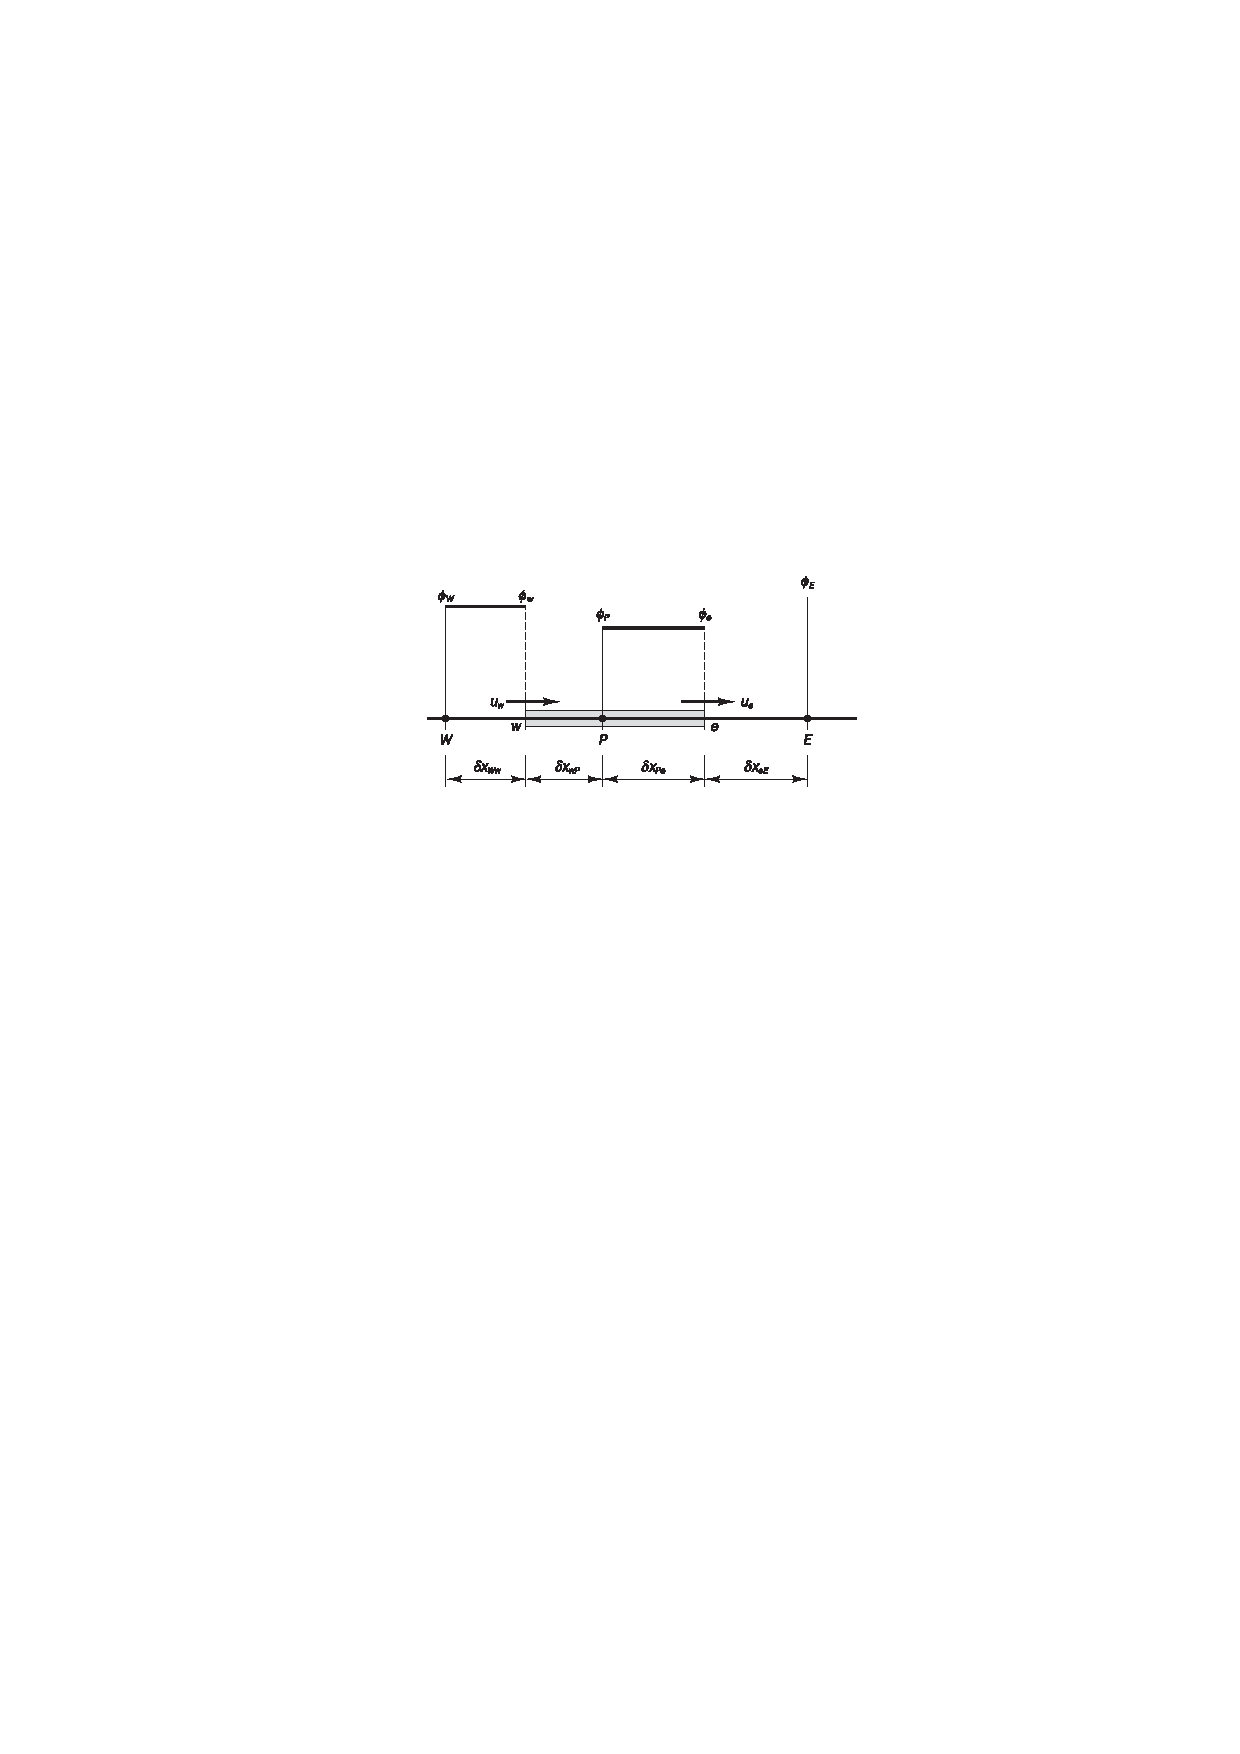
\includegraphics[scale=1.2]{images/52.pdf}
\caption{Upwind Differencing Scheme, in positive Direction (w)}
\label{fig:52}
\end{center}
\end{figure}
Bei der UDS-Interpolation wird der unbekannte Wert $\phi_f$ durch den bekannten
Wert von $\phi$ im nächsten stromauf gelegenen Zentralknoten ersetzt.
Es gilt also:

\begin{align}
\phi_w = \phi_W \\
\phi_e = \phi_P
\end{align}

Die diskretisierte Formel wird deshalb zu:

\begin{align}
\boxed{F_e \phi_P-F_w \phi_W = D_e(\phi_E - \phi_P) - D_w(\phi_P - \phi_W)}
\end{align}

Analog dazu lässt sich die Formel herleiten, wenn der Fluss in negative
U-Richtung verläuft. $\Rightarrow$ Versteeg S. 146

\textit{Vorteile}: Die Eigenschaften Conservativeness , Boundedness (keine
Wiggles) und Transportiveness (Richtung des Flusses) werden erfüllt. \\
\textit{Nachteile}: Numerische Accuracy (Das Schema basiert auf der
Backward Differencing Formel. Die Genauigkeit ist also nur erste Ordnung.) Wenn
der Fluss nicht synchron mit dem Netz verläuft, produziert das Schema
diffusionsartige Fehler. In Bild \ref{fig:54} ist eine solche Problemstellung
abgebildet. In Abbildung \ref{fig:53} die berechneten Resultate.

\begin{figure}[h!]
\begin{center}
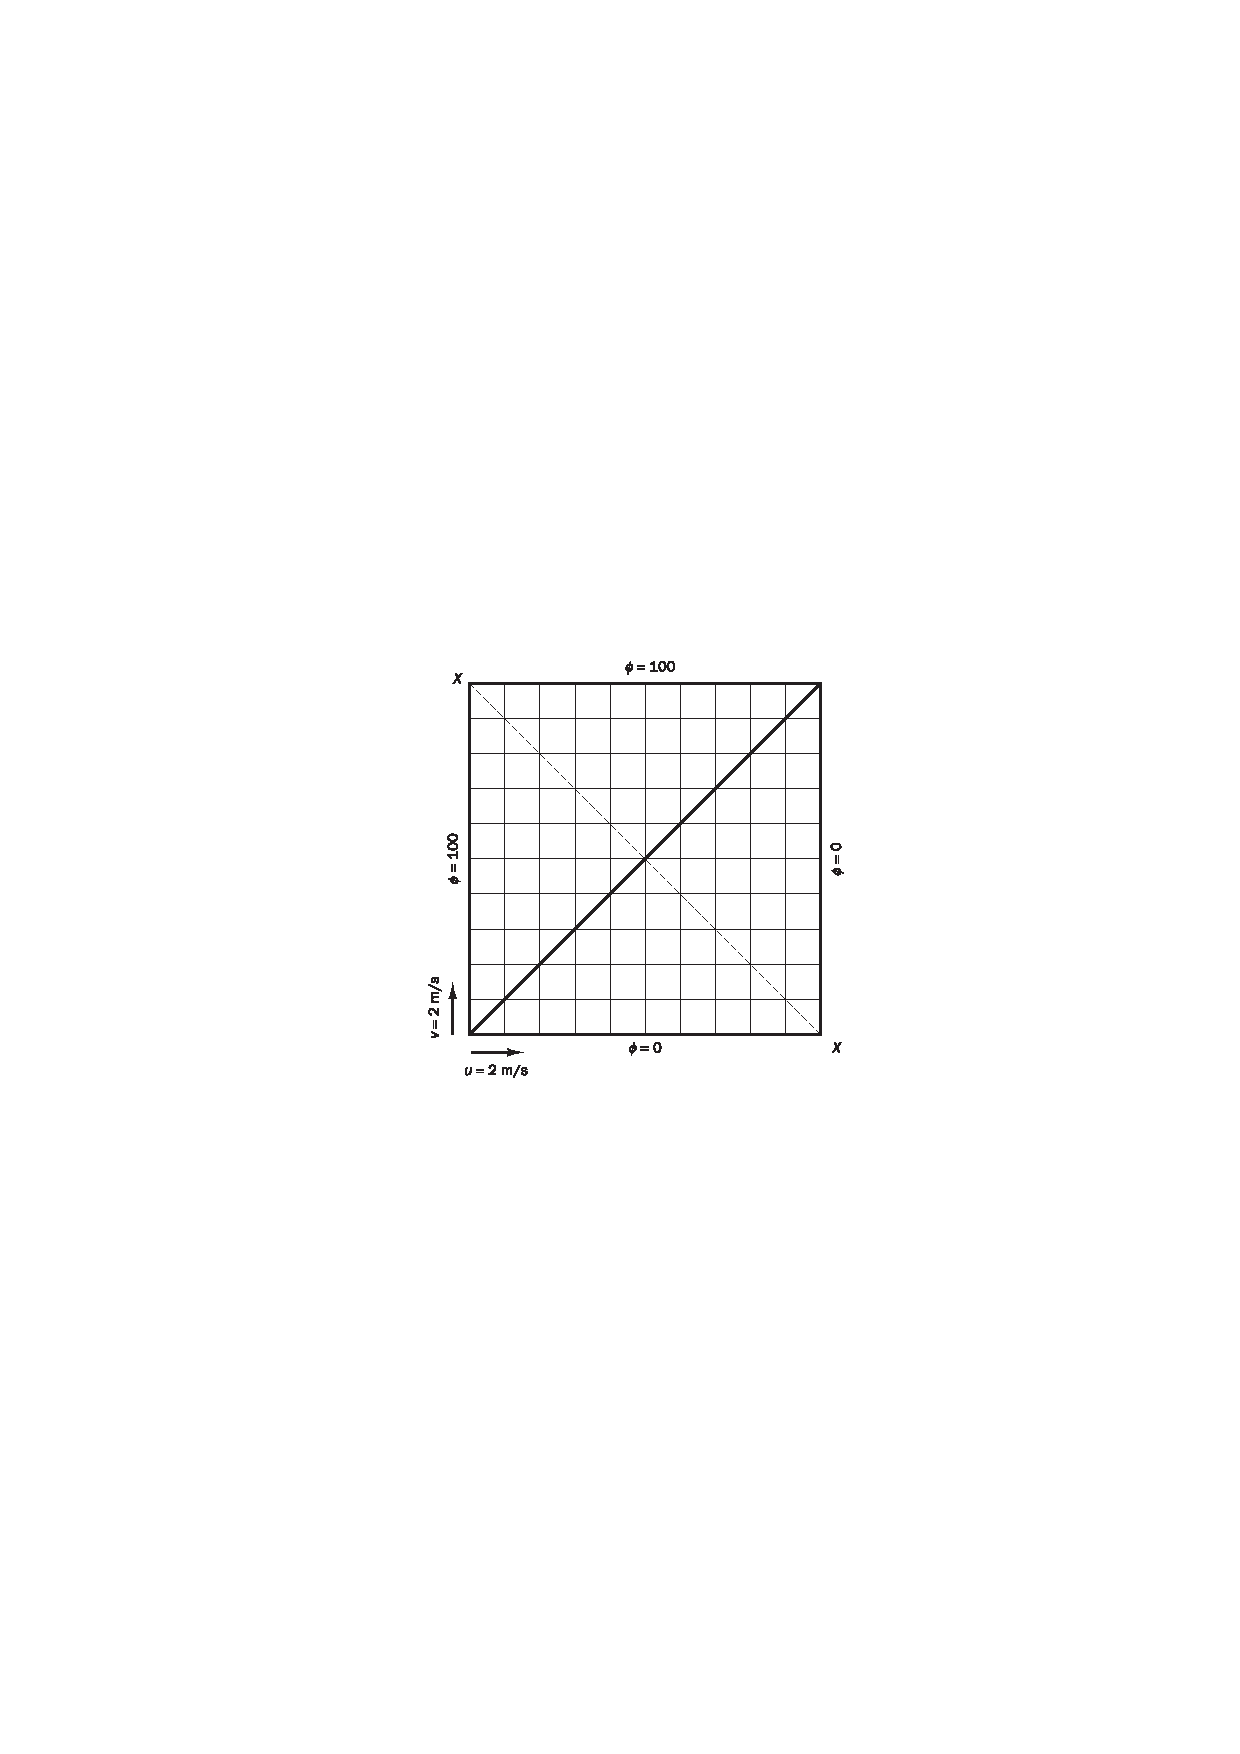
\includegraphics[scale=1.0]{images/54.pdf}
\caption{UDS Problemstellung, nicht an das Grid angepasster Fluss}
\label{fig:54}
\end{center}
\end{figure}

\begin{figure}[h!]
\begin{center}
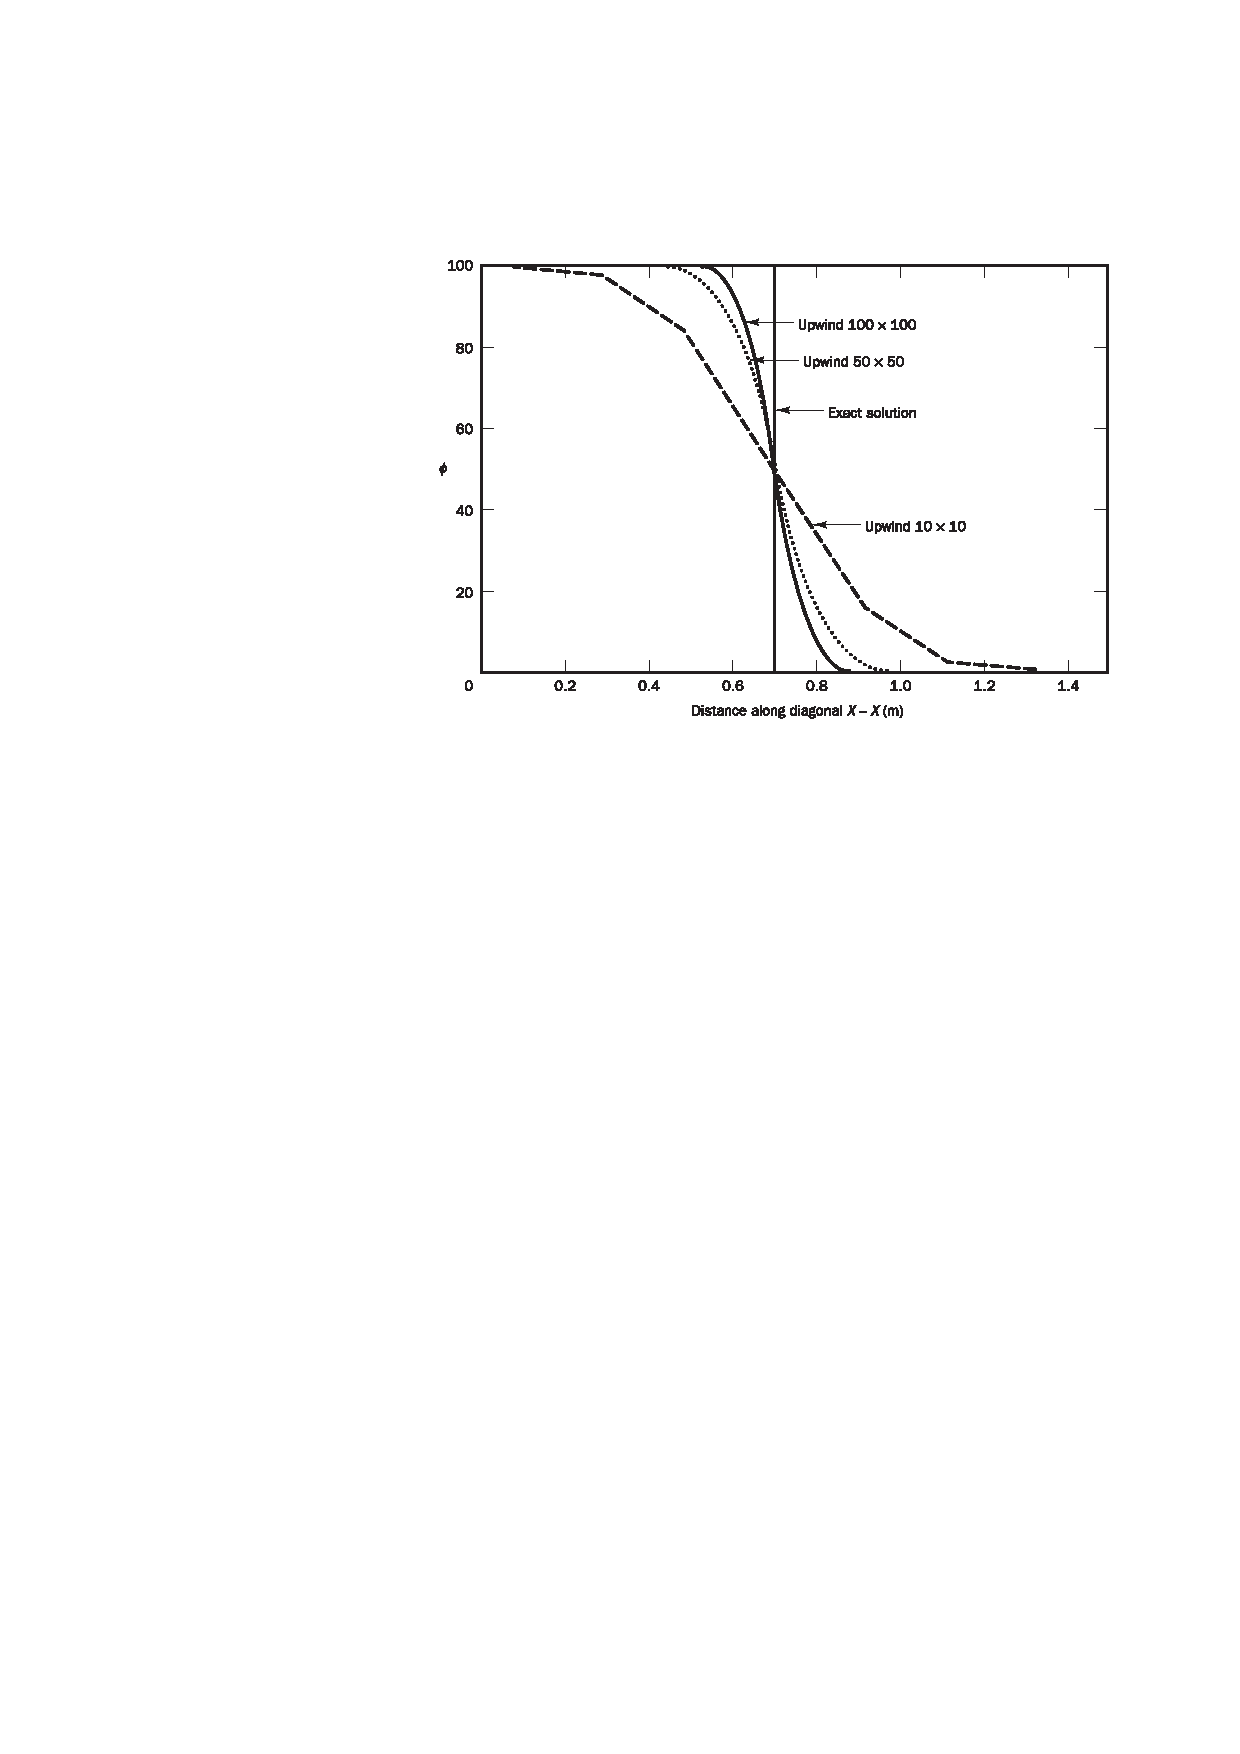
\includegraphics[scale=1.0]{images/53.pdf}
\caption{UDS Problemstellung, nicht an das Grid angepasster Fluss}
\label{fig:53}
\end{center}
\end{figure}


\subsection{Conservativeness, Boundedness, Transportiveness}
\begin{itemize}
  \item \textbf{Conservativeness}: Die Flüsse über die Flächen der Zellen
  müssen diesselben sein, also rechts und links: Der ganze Fluss der eine Zelle
  verlässt muss in eine neue Zelle eintreten.
  \item \textbf{Boundedness}: 
  \begin{itemize}
    \item Matrizen sollten diagonaldominant sein.$\Rightarrow$ Versteeg S.143
    \item Die Lösung sollte zwischen den gegebenen Randwerten liegen. Also wenn
    T(0)=100K und T(10)=200K gilt, sollen alle Lösungen dazwischen liegen.
    \item Alle Koeffizienten der Diskretisierung sollten positiv sein.
	\end{itemize}
\end{itemize}



\subsection{Hybrid Differencings} Explain how the hybrid differencing scheme
works.
idea: kombination von upwind und central, 1 Ordnung....
upwind: hoche PeKlee Zahen (hohe konvektion und wenig diffusion)
centrel diffenzing: kleine PeKlee Zahlen (weil mehr diffusion)

\subsection{Quick Scheme} Explain the QUICK scheme. Advantages and
disadvantages.
optimierung von upwind, schaut noch weiter in Zukunft und gewichtet die Zukunft
sehr negativ ist es überschwingt, dies ist total unphysikalisch
positiv näher an der exakten lösung




\subsection{TVD Schemes} Describe the idea behind TVD schemes.
TVD steht für Total Vaariation Diminishing,
Ideeist die Hügel zu reduzieren
Folie 19


\colorbox{red}{Domi macht}


\section{Solution algorithms for pressure velocity coupling in steady flows}
\subsection{Difference between incompressible and compressible approach}
Difference between incompressible (pressure-based) and compressible (density based) approach/codes => which equations are available for which variable
incompressibel, dichteänderung gleich 0 und p ist konstant
compressible, dichteänderung ...
folen 7


\subsection{Differences between momentum equations and general scalar transport
equations} 
Differences between momentum equations and general scalar transport
equations => new aspects to be tackled ??? zu folie 11

\subsection{SIMPLE}
Explain the SIMPLE procedure for pressure-velocity coupling\\
\newline
SIMPLE: Semi-Implicit Method for Pressure Linked Equations\\
Introinformationen (Wiki):\\
Der SIMPLE-Algorithmus (Semi-implicit Method for Pressure Linked Equations) wird
in der numerischen Strömungsmechanik zur Lösung der Navier-Stokes-Gleichungen
bei \textbf{unbekanntem Druckfeld} eingesetzt.\\
Die Grundidee, auf der SIMPLE basiert, ist das unbekannte Druckfeld zu schätzen,
die Geschwindigkeitsfelder damit zu berechnen und mit Hilfe der
Kontinuitätsgleichung eine Druckkorrektur und anschließend eine
Geschwindigkeitskorrektur zu bestimmen. Dieses Vorgehen wird wiederholt, bis die
Kontinuitätsgleichung im Rahmen der vorgegebenen Genauigkeit erfüllt wird.\\
\textbf{Iterativ} (wiä endlosschleifä, aber eifach ganz andersch)\\

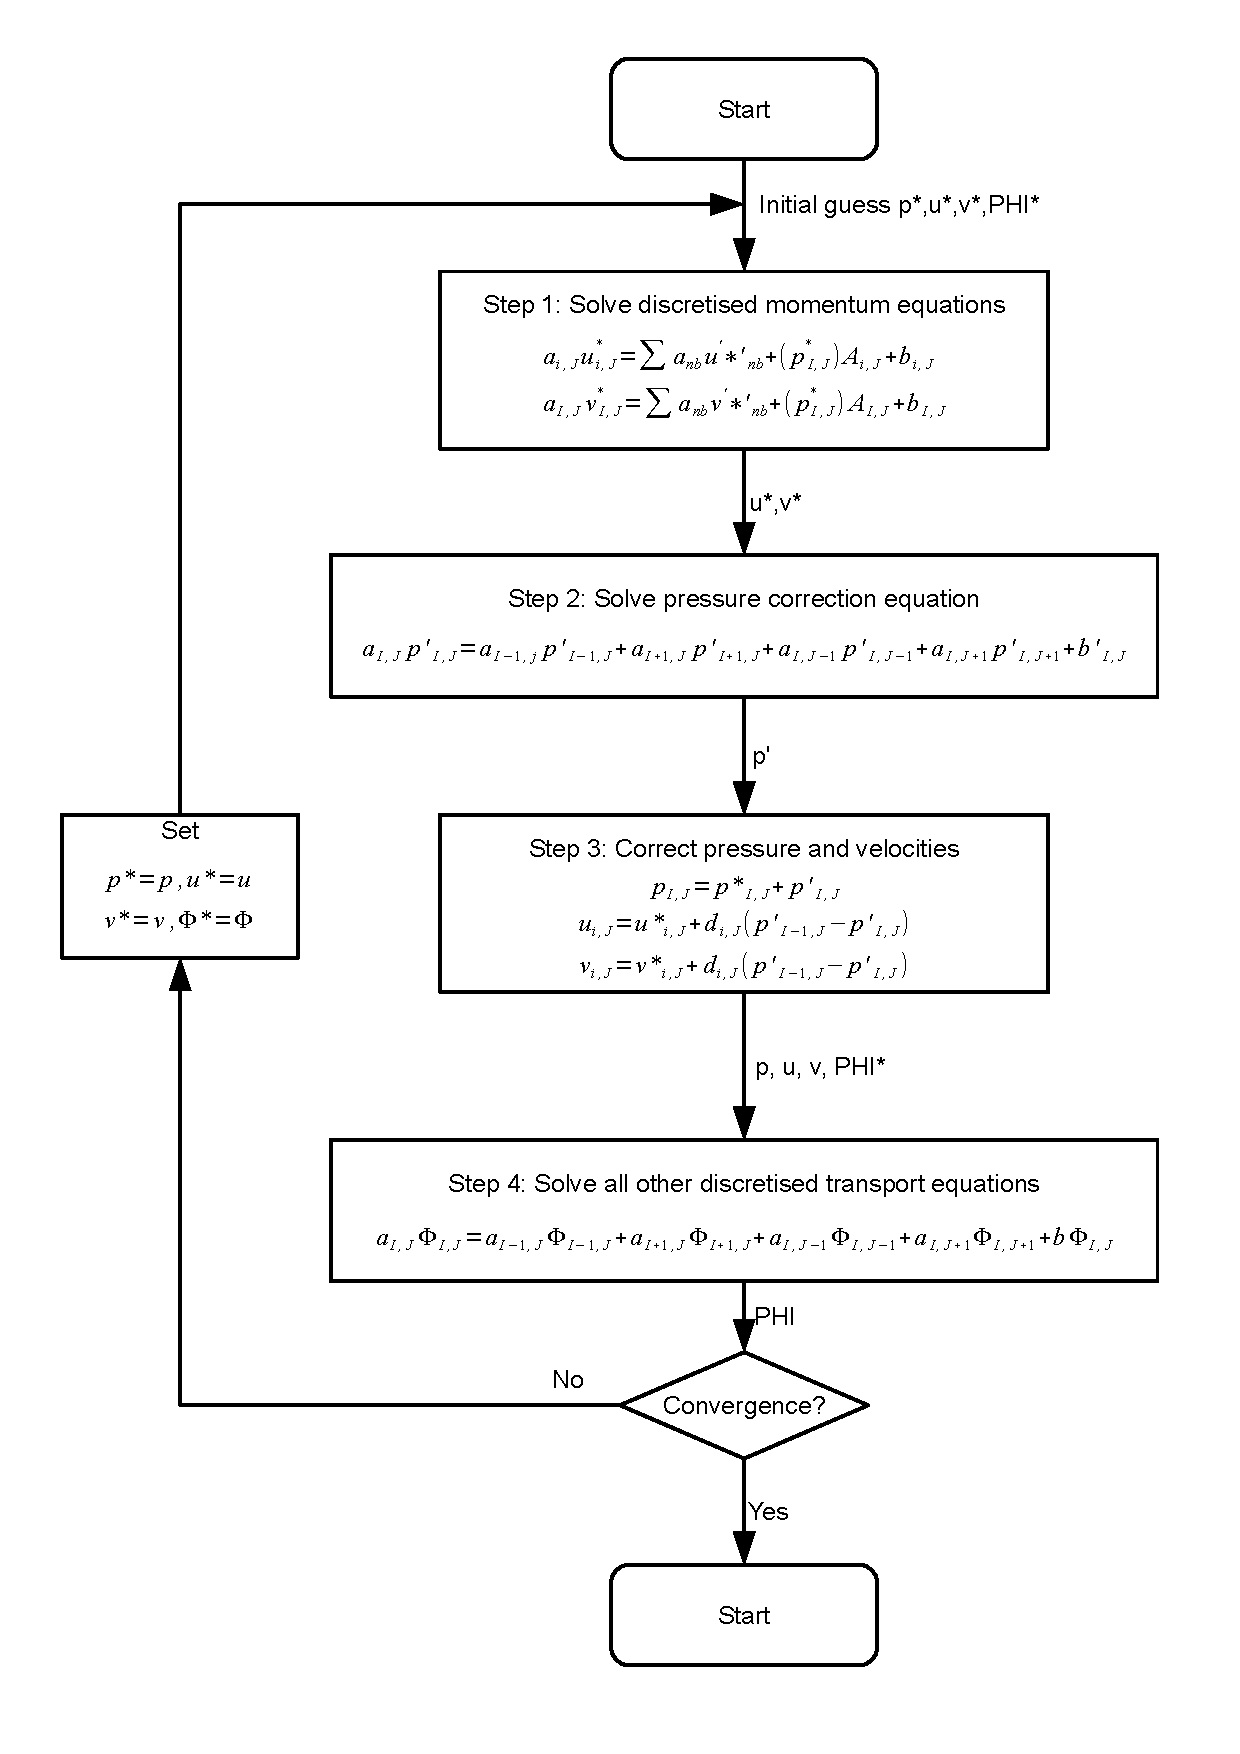
\includegraphics[scale=0.7]{images/simple_algorithm.pdf}\\
Kurz in Worte:\\
\begin{itemize}
  \item Iterationsprozess starten mit geschätzter Geschwindigkeit und Druckfeld
  \item Konvektiver Fluss durch die Zelloberfläche wird anhand der
  Geschwindigkeit abgeschätzt
  \item Geschätztes Druckfeld wird für die Lösung der Impulsgleichung verwendet
  \item Druckkorrekturgleichung, aus Kontinuitätsgleichung hergeleitet, um die
  Durckkorrektur zu berechnen. Anhand dieser wieder die Geschwindigkeit und
  Druckfeld berechnet wird.
  \item Es wird solange iteriert bis die Resultate des Geschwindigkeits und
  Druckfeld konvergieren (genügend genau sind)
\end{itemize}

Zusatzinfos:\\
\begin{itemize}
  \item Koeffizienten a werden durch Methoden (Central, hybrid, upwind, quick,
  \ldots) berechnet
  \item $d_{i,J} = \frac{A_{i,J}}{a_{i,J}}$ und $d_{I,J} =
  \frac{A_{I,J}}{a_{I,J}}$
  \item Druck: p
  \item Geschwindigkeitskomponenten: u, v
\end{itemize}

Branches von Simple:\\
\begin{itemize}
  \item SIMPLER (R for revised, Patankar, 1980): In this algorithm the
  continuity equation is used to derive a pressure instead of a pressure correction equation as in SIMPLE. The intermediate pressure field is obtained directly without the use of a correction. Velocities are, however, still obtained through the velocity corrections as in SIMPLE
  \item SIMPLEC (C for consistent, van Doormal-Raithby, 1984): this algorithm
  follows the same steps as the SIMPLE algorithm, but the momentum equations are manipulated so that the SIMPLEC velocity correction equations omit terms that are less significant than those in SIMPLE
  \item PISO (Pressure Implicit with Splitting of Operators, Issa, 1986): is a
  p–v calculation procedure developed originally for non-iterative computation of unsteady compressible flows. It has been adapted successfully for the iterative solution of steady state problems. PISO involves one predictor step and two corrector steps and may be seen as an extension of SIMPLE, with a further corrector step to enhance it
\end{itemize}

Beschrieben in Lektion 7, Pressure Velocity Coupling: Folie 14


\subsection{Relaxation Factor and Uses of it}
Explain the role of relaxation factor. 
Flussdiagramm siehe Folie 14
 Why are they used?
folie 20
\colorbox{red}{Bischi macht}


\section{Solution of discretized equations}


\subsection{Iterative methods} 
Explain why iterative methods are necessary to
solve sparse linear systems.
schneller gelöst, numerisch weniger aufwindig
Iterative löser ...
sparse linear system sind einfach pararellisierbar viele Nullen

Rechenzeitenverglich Tabelle erstellen

\subsection{Jacobi and Gauss-Seidel iterative methods}
Describe the Jacobi and Gauss-Seidel iterative methods
Jacobi iterative method: 
möglichst nahe an einheitsmatix kommen
eigenwert muss keiner 1 sein das es konvergiert, wird dafür langsamer 
gut paararellisierbar

Gauss- Seidel method: 
nicht paararellisierbar, konvergit schneller

\subsection{Multi-Grid Methods} 
Describe the idea behind the multi-grid method
Anfangsbedingungne 
Stufenweises lösen auf verschiednen netzgrüssen
foleie 19 (Ansys arbeitet so)
feien lösen
grobes netzt lösen
dann wieder feiner...
im Buch lesen auf deutsch... seite 82

\colorbox{red}{Simon}

\section{The finite volume method for unsteady flows}
\subsection{Common Schemes} Describe the three common schemes for time
discretization:

Einehitskreis 
\begin{itemize}
\item Explicit (forward Euler)
...

\item Cranck-Nicholson $\Rightarrow$ CDS
Könnte Schwingen
...

\item Implicit (backward Euler)
...

\end{itemize}
\subsection{Advantages and disadvantages of the different schemes}
\begin{itemize}
\item Explicit (forward Euler)
Schnell

\item Cranck-Nicholson
Instabil, aber genau

\item Implicit (backward Euler)
Robust 
\end{itemize}
\subsection{SIMPLE scheme}
How does the SIMPLE scheme have to be modified for a transient
simulation?

\colorbox{red}{Domi}


\section{Implementation of boundary conditions}


\subsection{5 important boundary conditions}

 Name 5 important boundary
conditions Dirichlet boundary conditions
Neumann boundary conditions
Robin bandary  condition


inelt
outlet
wall



\subsection{Why cannot symmetry planes (and symmetry boundary conditions always
be used in CFD)?}
Why cannot symmetry planes (and symmetry boundary conditions always
be used in CFD)
\subsection{Why should outlets be placed far away from the interesting flow
region?}
 weil am anfang am rand falsche randbedingungen sind, siehe bild silvio,
slide 38

\colorbox{red}{Bischi}

\section{Errors and uncertainty in CFD modelling}

\subsection{3 potential numerical errors in CFD}

Describe three potential numerical errors in CFD
\begin{itemize}
\item \textbf{Disketierungsfehler}: Netz musste unendlich fein sein, um die physikalische Effekte aufzulösen. Aus diesem Grund ist es notwendig verschiedenen Netzen und Zeitschritten eine Netzstudie durchzuführen, so Resultat dasselbe Effekte gibt
\item \textbf{Rundungsfehler}: Bei Gleitkommazahlen können beim rechnen mit dem Computer Fehler entstehen, dies weil Teile davon beim Rechnen verloren  gehen Meist mit Float.h kann nachgeschaut werden.
\item \textbf{Iterative}: Konvergenzfehler, wenn Residuale welche beim Lösen entstehen nicht stimmen, stimmt die Physik sicher nicht.  
\end{itemize}

\subsection{Two typical physical uncertainties in CFD}
Describe two typical physical uncertainties in CFD (uncertainties =
Unsicherheiten)
\begin{itemize}
\item \textbf{limitierte Genauigkeit}
\item \textbf{fehlen von validierten Submodellen}
\end{itemize}
weitere Informationen im Buch Versteeg Seite 291

\subsection{Verification and Validation} 
What do the terms verification and
validation mean.
\begin{itemize}
\item \textbf{Verification}: Aufgabe des Mathematiker, schaut das die Gleichung richtig gelöst wird.
\item \textbf{Validation}: Aufgabe des Ingenieur, schaut das die richtige Gleichung gelöst wird, welche die Wirklichkeit beschreibt.
\end{itemize}


\colorbox{red}{Simon}





\end{document}




